\documentclass[12 pt]{article}
\usepackage{amsmath}
\usepackage{url}
\usepackage{graphicx}
\usepackage{setspace}
\usepackage{pgf}
\usepackage{tikz}
\usetikzlibrary{arrows,automata}
\usepackage[latin1]{inputenc}
\usepackage{verbatim}
\usepackage{lscape}
%\usepackage[margin=1.2in]{geometry}

	\addtolength{\oddsidemargin}{-.5in}
	\addtolength{\evensidemargin}{-.5in}
	\addtolength{\textwidth}{0.75in}
	\addtolength{\topmargin}{-1in}
	\addtolength{\textheight}{1.75in}
\begin{document}

\newcommand{\vocab}{\mathbf{v}}
\newcommand{\dtvec}{\mathbf{t}_\Delta}
\newcommand{\ctxvec}{\mathbf{t}_\text{ctx}}
\newcommand{\dt}{\Delta_t}
\newcommand{\prerror}{Pr_{error}}

\section{Method}

Extract data collected from forums Timestamp, Author, Text Content. Using sliding window training method, group consecutive $w$ posts together and perform regression on $\dt$. More formally, we are trying to learn a function $f$ such that $f(\mathbf{x}_{t-w},\hdots, \mathbf{x}_{t-1}) \approx \Delta_{t}$, where $\mathbf{x}_t$ is the feature vector of a post made at time $t$, and $\dt$ is the time between the $t$-th post and the $(t-1)$-th post. The following are the features used:
\begin{description}
	\item[Previous time differences] All the time differences between posts made in the window. ($\dtvec$)
	\item[Time-based features] Day of week, Hour of day. Provides contextual information about when the post was made. ($\ctxvec$)
	
	\item[Content features (text)]
		Word frequency counts are used for this set of experiments. Using regression, we find the top $K$ variables that the actual $\dt$ depends on. Table \ref{vocab_exp} reflect the results of the experiments done with varying values of $K$.

\end{description}


\begin{table}
	\footnotesize
	\begin{centering}
	\begin{tabular}{|l|c|c|c|c|c|c|c|c|}
	\hline
	\input{vocab_exp}
	\hline
	\end{tabular}
	\caption{Experiment results: Varying vocabulary size}
	\label{vocab_exp}
\end{centering}
\end{table}



In the following experiments, the threads chosen from our extracted dataset are those with a 100 to 1000 posts. This amounted to 97 threads. The first 75\% of the thread was used as training data, while the remaining 75\% was used as test data. We used Support Vector machines for this regression task, employing a Radial Basis Function kernel as our learning algorithm. 

The SVR module from the Python library scikit-learn was used in the implementation of this experiment.


%include diagrams

\subsection{Evaluation metrics}
We use \emph{Mean Absolute Percentage Error} (MAPE), to measure the performance of the learnt model. This value is given by
\[
	\frac{1}{N}\sum^N_{i=1}\left|\frac{A_i-F_i}{A_i}\right|
\]
where $A_i$ is the actual value, and $F_i$ is the forecasted value for the instance $i$. Realistically, the model would not be able to come into contact with every possible window, since chances are it will make an error that causes %explain error in a new section (before this one) ?
it to visit a thread late, causing it to miss two posts or more. This value does not reflect how well the model will do in a real-time setting, but gives an idea of how far off the model is given a window. 

We also want to know the \emph{timeliness} of the model's visits. Yang et. al. \cite{Yang2009} has a metric for measuring this. Taking $\Delta t_i$ as the time difference between a post $i$ and it's download time, the timeliness of the algorithm is given by
\[T = \frac{1}{N} \sum^{N}_{i=1}\Delta t_i\]
A good algorithm would give a low $T$-score. However, a crawler that hits the site repeatedly performs well according to this metric. The authors account for this by setting a bandwidth (fixed number of pages per day) for each iteration of their testing. In our experimental results, we also take into account the number of page requests made in comparison to the number of posts. %ratio?

Viewing the posts made during the thread's lifetime as segmentations of the thread, and the visits made as hypotheses of where the segmentations are, we use the $\prerror$ metric from Georgescul et. al., 2006 as a measure of how close the predictions are to the actual posts. An example can be seen in Figure \ref{prerror}.


\begin{figure}
\[
	\uparrow~~p_1,\underbrace{~~p_2,~~p_3,~~~p_4,\uparrow}_{\text{sliding window}}\uparrow
\]
\caption{An example of the sliding window metric. The metric is made up of two components: First, the probability that, given at least one post is present in the window, there are more visits than post. Secondly, the probability that there are more posts than visits for a given window. The weighted sum of this gives the overall $\prerror$}\label{prerror}
\end{figure}

\section{Results}

The results for experiments done with different combinations of the above specified features are shown in Table \ref{expt1}.
\begin{table}
	\footnotesize
	\begin{centering}
	\begin{tabular}{|l|c|c|c|c|c|c|c|c|}
	\hline
	\input{init_res}
	\hline
	\end{tabular}
	\caption{Experiment results}
	\label{expt1}
\end{centering}
\end{table}

Overall average and window average perform significantly worst than the learnt models, as reflected in both the MAPE and the $T$-score. There is also a slight improvement in the  $\prerror$ in the learnt models.


Taking into account the $T$-score and the number of visits together, would seem that $\dtvec$, features representing the previous time intervals, are important features when determining the next time interval. In the absence of these features, we observe that the $T$-score increases by about 1\%. In this experiment, we use purely word frequency features. This gives only a slight improvent over not using them.

High values for $Pr_{miss}$ and low for $Pr_{fa}$, are due to $Pr_{miss}$ being conditioned on there being a post within the window. Since the posts come in bursts, visits are fairly periodic, and intervals between visits are larger than post bursts. When there are more posts than visits in windows with posts, we have higher $Pr_{miss}$

\begin{landscape}
\begin{figure}
	\centering
	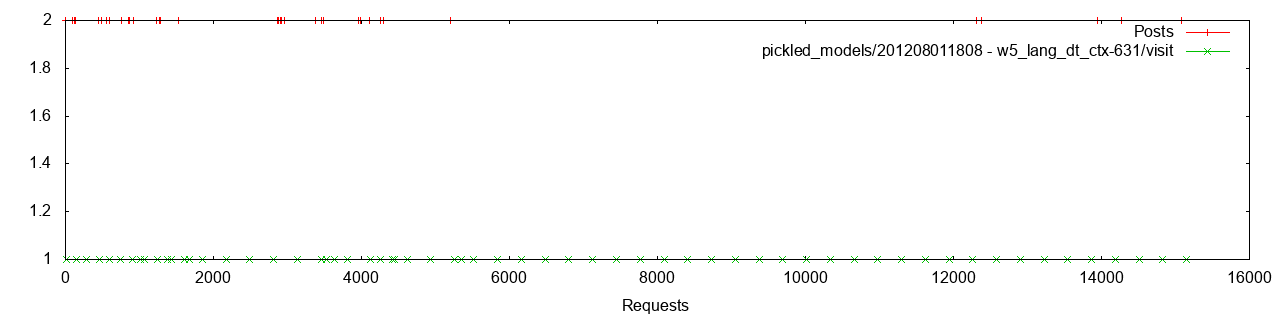
\includegraphics[scale=0.5]{example_seq.png}
	\caption{Visitation chart for a model using the $w=5, \mathbf{t}_\Delta, \mathbf{t}_{\text{ctx}},\mathbf{w}$ feature set. Invalid Predictions = 0.758, $Pr_{error} =  0.485$, $T$-score = 119.612, Posts = 41, Visits = 62}
\end{figure}
\end{landscape}

\begin{table}
	\footnotesize
	\begin{centering}
	\begin{tabular}{|l|c|c|c|c|c|c|c|c|}
	\hline
	\input{f_size}
	\hline
	\end{tabular}
	\caption{Experiment results: Varying feature sizes}
	\label{exp_f_size}
\end{centering}
\end{table}


\bibliographystyle{acm}
\bibliography{report}
\end{document}
